\documentclass[10pt, a5paper]{article}
\usepackage{pdfpages}
\usepackage{parallel}
\usepackage[T2A]{fontenc}
\usepackage{ucs}
\usepackage[utf8x]{inputenc}
\usepackage[polish,english,russian]{babel}
\usepackage{hyperref}
\usepackage{rotating}
\usepackage[inner=2cm,top=1.8cm,outer=2cm,bottom=2.3cm,nohead]{geometry}
\usepackage{listings}
\usepackage{graphicx}
\usepackage{wrapfig}
\usepackage{longtable}
\usepackage{indentfirst}
\usepackage{array}
\newcolumntype{P}[1]{>{\raggedright\arraybackslash}p{#1}}
\frenchspacing
\usepackage{fixltx2e} %text sub- and superscripts
\usepackage{icomma} % коскі ў матэматычным рэжыме
\PreloadUnicodePage{4}

\newcommand{\longpage}{\enlargethispage{\baselineskip}}
\newcommand{\shortpage}{\enlargethispage{-\baselineskip}}

\def\switchlang#1{\expandafter\csname switchlang#1\endcsname}
\def\switchlangbe{
\let\saverefname=\refname%
\def\refname{Літаратура}%
\def\figurename{Іл.}%
}
\def\switchlangen{
\let\saverefname=\refname%
\def\refname{References}%
\def\figurename{Fig.}%
}
\def\switchlangru{
\let\saverefname=\refname%
\let\savefigurename=\figurename%
\def\refname{Литература}%
\def\figurename{Рис.}%
}

\hyphenation{admi-ni-stra-tive}
\hyphenation{ex-pe-ri-ence}
\hyphenation{fle-xi-bi-li-ty}
\hyphenation{Py-thon}
\hyphenation{ma-the-ma-ti-cal}
\hyphenation{re-ported}
\hyphenation{imp-le-menta-tions}
\hyphenation{pro-vides}
\hyphenation{en-gi-neering}
\hyphenation{com-pa-ti-bi-li-ty}
\hyphenation{im-pos-sible}
\hyphenation{desk-top}
\hyphenation{elec-tro-nic}
\hyphenation{com-pa-ny}
\hyphenation{de-ve-lop-ment}
\hyphenation{de-ve-loping}
\hyphenation{de-ve-lop}
\hyphenation{da-ta-ba-se}
\hyphenation{plat-forms}
\hyphenation{or-ga-ni-za-tion}
\hyphenation{pro-gramming}
\hyphenation{in-stru-ments}
\hyphenation{Li-nux}
\hyphenation{sour-ce}
\hyphenation{en-vi-ron-ment}
\hyphenation{Te-le-pathy}
\hyphenation{Li-nux-ov-ka}
\hyphenation{Open-BSD}
\hyphenation{Free-BSD}
\hyphenation{men-ti-on-ed}
\hyphenation{app-li-ca-tion}

\def\progref!#1!{\texttt{#1}}
\renewcommand{\arraystretch}{2} %Іначай формулы ў матрыцы зліпаюцца з лініямі
\usepackage{array}

\def\interview #1 (#2), #3, #4, #5\par{

\section[#1, #3, #4]{#1 -- #3, #4}
\def\qname{LVEE}
\def\aname{#1}
\def\q ##1\par{{\noindent \bf \qname: ##1 }\par}
\def\a{{\noindent \bf \aname: } \def\qname{L}\def\aname{#2}}
}

\def\interview* #1 (#2), #3, #4, #5\par{

\section*{#1\\{\small\rm #3, #4. #5}}

\def\qname{LVEE}
\def\aname{#1}
\def\q ##1\par{{\noindent \bf \qname: ##1 }\par}
\def\a{{\noindent \bf \aname: } \def\qname{L}\def\aname{#2}}
}

\switchlang{ru}
\begin{document}
\title{Сизиф на Эльбрусе: следующая станция}
\author{Михаил Шигорин, Москва, Россия\footnote{\url{mike@altlinux.org}, \url{http://lvee.org/ru/abstracts/314}}}
\maketitle
\begin{abstract}
Yes, we're rolling ALT p9 out with Elbrus support among the multitude of new primary and secondary platforms.
\end{abstract}
\section*{Девятая платформа}

Три года назад мой доклад был про выпуск восьмой платформы ALT; пришла пора и для девятой.  На этот раз мы делаем выпуск не только для 64/32-битных x86, но и для 64-битных ARM/Power в качестве основных платформ с обеспечением синхронной сборки в репозиторий, а также 64-битного RISC-V и 32-битных ARM/MIPSel в догоняющем режиме --- но для меня наиболее интересной новинкой является, конечно, доступность девятой платформы Альт на процессорах <<Эльбрус>> третьего и четвёртого поколения.
В сумме это всё даёт разработчикам и пользователям широчайшие возможности применения отечественных и перспективных мировых аппаратных архитектур при необходимости или желании отказаться от наследственной x86 со всем её грузом проблем (хотя стоит понимать, что такой груз разменивается на иной, а не исчезает).

\section*{Пакеты, версии, возможности}

Что нового по сравнению с прошлогодним выпуском, причисленным к восьмой платформе, но основанным на примерно среднем между p8 и p9 состоянии Сизифа, нашего репозитория разработки?

Разумеется, главное --- переход на новую ветку компилятора LCC: с 1.21 на 1.23.  Это дало базовую совместимость с GCC 5.5 вместо 4.8.0, в т.ч. поддержку C++11 (и частично C++14), а также несколько возросшую производительность собранного кода на том же оборудовании плюс возможность оптимизировать как под выбранное поколение, так и под конкретный процессор.

Обновлены и другие трансляторы, включая perl 5.28 с python 3.7; подтянут и сборочный инструментарий, в т.ч. meson 0.50 и cmake 3.11.  Также набор языков пополнился LISP (clisp, picolisp), R и базовым OCaml.  Разумеется, пополнились и обновились библиотеки, прикладные и серверные пакеты --- например, наконец-то осуществлён переход на единую Samba 4.10 вместо <<обычной>> и DC-сборок, Qt обновлена до 5.9, а список десктопных окружений пополнился Cinnamon 4.2.

Ну и тихо-незаметно обновили менеджер пакетов RPM до 4.13, а ядро Linux --- до 4.9 (над 4.19 в МЦСТ пока трудятся).

На \href{http://packages.altlinux.org}{packages.altlinux.org} добавлены сведения по наличию и версиям пакетов для e2k, а также их spec-файлы.

\section*{Формы распространения}

\noindent Наши наработки доступны теперь не только после установки обычных дистрибутивов <<Альт Сервер>> (\href{http://basealt.ru/products/alt-server}{basealt.ru/products/alt-server}) и <<Альт Рабочая станция>> (\href{http://basealt.ru/products/alt-workstation}{basealt.ru/products/alt-workstation}) в вариантах для Эльбруса, но и в добравшихся и сюда стартовых наборах.

К сожалению, работы поставщика по публикации набора разработчика под платформу Эльбрус (\url{http://mcst.ru/elbrus_pdk}) (PDK) пока не завершены и наши образы/репозитории тоже не могут быть выложены публично (доступны только покупателям соответствующего оборудования) --- но есть надежда на скорое улучшение этой ситуации.

Тем временем мы начали публикацию внутренних заметок и прочего полезного архитектурнозависимого знания в разделе вики \href{http://altlinux.org/elbrus}{altlinux.org/elbrus}.

\begin{center}
\begin{figure}[h!]
  \centering
  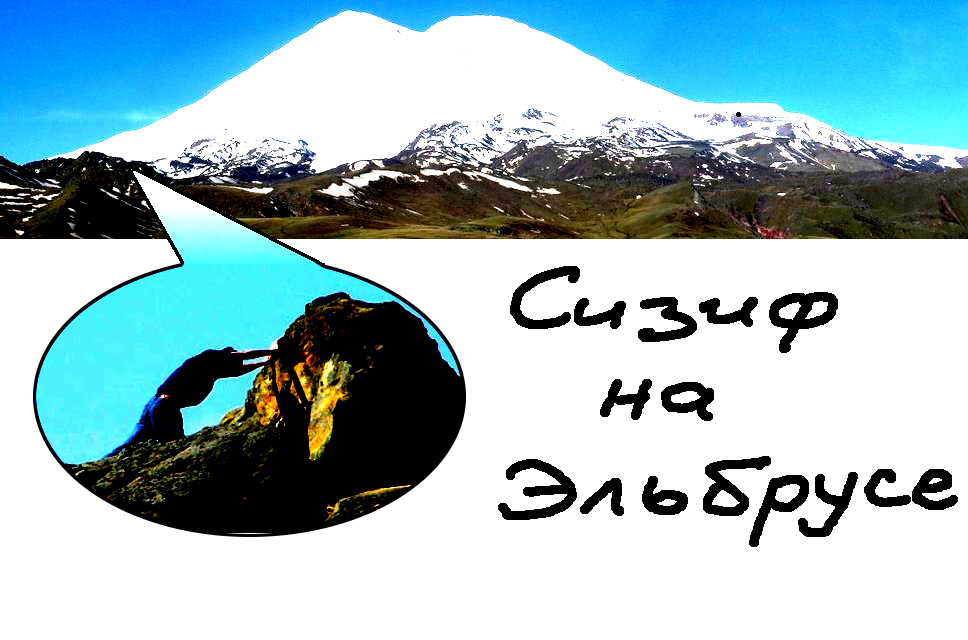
\includegraphics[width=10.8cm]{2019_Shigorin.png}

  \label{fig1}
\end{figure}
\end{center} 

\section*{Будни}

В общем, прорывов всё меньше, планомерной работы всё больше --- как и начинающих давать отдачу результатов её применения.
Кстати, я опять ищу помощников --- и спасибо LVEE за то, что Андрей Савченко уже откликнулся и вложил немало трудов в то, чтобы озвученное состоялось :)


\end{document}
